% Options for packages loaded elsewhere
\PassOptionsToPackage{unicode}{hyperref}
\PassOptionsToPackage{hyphens}{url}
\PassOptionsToPackage{dvipsnames,svgnames,x11names}{xcolor}
%
\documentclass[
  letterpaper,
  DIV=11,
  numbers=noendperiod,
  oneside]{scrartcl}

\usepackage{amsmath,amssymb}
\usepackage{iftex}
\ifPDFTeX
  \usepackage[T1]{fontenc}
  \usepackage[utf8]{inputenc}
  \usepackage{textcomp} % provide euro and other symbols
\else % if luatex or xetex
  \usepackage{unicode-math}
  \defaultfontfeatures{Scale=MatchLowercase}
  \defaultfontfeatures[\rmfamily]{Ligatures=TeX,Scale=1}
\fi
\usepackage{lmodern}
\ifPDFTeX\else  
    % xetex/luatex font selection
\fi
% Use upquote if available, for straight quotes in verbatim environments
\IfFileExists{upquote.sty}{\usepackage{upquote}}{}
\IfFileExists{microtype.sty}{% use microtype if available
  \usepackage[]{microtype}
  \UseMicrotypeSet[protrusion]{basicmath} % disable protrusion for tt fonts
}{}
\makeatletter
\@ifundefined{KOMAClassName}{% if non-KOMA class
  \IfFileExists{parskip.sty}{%
    \usepackage{parskip}
  }{% else
    \setlength{\parindent}{0pt}
    \setlength{\parskip}{6pt plus 2pt minus 1pt}}
}{% if KOMA class
  \KOMAoptions{parskip=half}}
\makeatother
\usepackage{xcolor}
\usepackage[left=1in,marginparwidth=2.0666666666667in,textwidth=4.1333333333333in,marginparsep=0.3in]{geometry}
\ifLuaTeX
  \usepackage{luacolor}
  \usepackage[soul]{lua-ul}
\else
  \usepackage{soul}
  
\fi
\setlength{\emergencystretch}{3em} % prevent overfull lines
\setcounter{secnumdepth}{-\maxdimen} % remove section numbering
% Make \paragraph and \subparagraph free-standing
\ifx\paragraph\undefined\else
  \let\oldparagraph\paragraph
  \renewcommand{\paragraph}[1]{\oldparagraph{#1}\mbox{}}
\fi
\ifx\subparagraph\undefined\else
  \let\oldsubparagraph\subparagraph
  \renewcommand{\subparagraph}[1]{\oldsubparagraph{#1}\mbox{}}
\fi

\usepackage{color}
\usepackage{fancyvrb}
\newcommand{\VerbBar}{|}
\newcommand{\VERB}{\Verb[commandchars=\\\{\}]}
\DefineVerbatimEnvironment{Highlighting}{Verbatim}{commandchars=\\\{\}}
% Add ',fontsize=\small' for more characters per line
\usepackage{framed}
\definecolor{shadecolor}{RGB}{241,243,245}
\newenvironment{Shaded}{\begin{snugshade}}{\end{snugshade}}
\newcommand{\AlertTok}[1]{\textcolor[rgb]{0.68,0.00,0.00}{#1}}
\newcommand{\AnnotationTok}[1]{\textcolor[rgb]{0.37,0.37,0.37}{#1}}
\newcommand{\AttributeTok}[1]{\textcolor[rgb]{0.40,0.45,0.13}{#1}}
\newcommand{\BaseNTok}[1]{\textcolor[rgb]{0.68,0.00,0.00}{#1}}
\newcommand{\BuiltInTok}[1]{\textcolor[rgb]{0.00,0.23,0.31}{#1}}
\newcommand{\CharTok}[1]{\textcolor[rgb]{0.13,0.47,0.30}{#1}}
\newcommand{\CommentTok}[1]{\textcolor[rgb]{0.37,0.37,0.37}{#1}}
\newcommand{\CommentVarTok}[1]{\textcolor[rgb]{0.37,0.37,0.37}{\textit{#1}}}
\newcommand{\ConstantTok}[1]{\textcolor[rgb]{0.56,0.35,0.01}{#1}}
\newcommand{\ControlFlowTok}[1]{\textcolor[rgb]{0.00,0.23,0.31}{#1}}
\newcommand{\DataTypeTok}[1]{\textcolor[rgb]{0.68,0.00,0.00}{#1}}
\newcommand{\DecValTok}[1]{\textcolor[rgb]{0.68,0.00,0.00}{#1}}
\newcommand{\DocumentationTok}[1]{\textcolor[rgb]{0.37,0.37,0.37}{\textit{#1}}}
\newcommand{\ErrorTok}[1]{\textcolor[rgb]{0.68,0.00,0.00}{#1}}
\newcommand{\ExtensionTok}[1]{\textcolor[rgb]{0.00,0.23,0.31}{#1}}
\newcommand{\FloatTok}[1]{\textcolor[rgb]{0.68,0.00,0.00}{#1}}
\newcommand{\FunctionTok}[1]{\textcolor[rgb]{0.28,0.35,0.67}{#1}}
\newcommand{\ImportTok}[1]{\textcolor[rgb]{0.00,0.46,0.62}{#1}}
\newcommand{\InformationTok}[1]{\textcolor[rgb]{0.37,0.37,0.37}{#1}}
\newcommand{\KeywordTok}[1]{\textcolor[rgb]{0.00,0.23,0.31}{#1}}
\newcommand{\NormalTok}[1]{\textcolor[rgb]{0.00,0.23,0.31}{#1}}
\newcommand{\OperatorTok}[1]{\textcolor[rgb]{0.37,0.37,0.37}{#1}}
\newcommand{\OtherTok}[1]{\textcolor[rgb]{0.00,0.23,0.31}{#1}}
\newcommand{\PreprocessorTok}[1]{\textcolor[rgb]{0.68,0.00,0.00}{#1}}
\newcommand{\RegionMarkerTok}[1]{\textcolor[rgb]{0.00,0.23,0.31}{#1}}
\newcommand{\SpecialCharTok}[1]{\textcolor[rgb]{0.37,0.37,0.37}{#1}}
\newcommand{\SpecialStringTok}[1]{\textcolor[rgb]{0.13,0.47,0.30}{#1}}
\newcommand{\StringTok}[1]{\textcolor[rgb]{0.13,0.47,0.30}{#1}}
\newcommand{\VariableTok}[1]{\textcolor[rgb]{0.07,0.07,0.07}{#1}}
\newcommand{\VerbatimStringTok}[1]{\textcolor[rgb]{0.13,0.47,0.30}{#1}}
\newcommand{\WarningTok}[1]{\textcolor[rgb]{0.37,0.37,0.37}{\textit{#1}}}

\providecommand{\tightlist}{%
  \setlength{\itemsep}{0pt}\setlength{\parskip}{0pt}}\usepackage{longtable,booktabs,array}
\usepackage{calc} % for calculating minipage widths
% Correct order of tables after \paragraph or \subparagraph
\usepackage{etoolbox}
\makeatletter
\patchcmd\longtable{\par}{\if@noskipsec\mbox{}\fi\par}{}{}
\makeatother
% Allow footnotes in longtable head/foot
\IfFileExists{footnotehyper.sty}{\usepackage{footnotehyper}}{\usepackage{footnote}}
\makesavenoteenv{longtable}
\usepackage{graphicx}
\makeatletter
\def\maxwidth{\ifdim\Gin@nat@width>\linewidth\linewidth\else\Gin@nat@width\fi}
\def\maxheight{\ifdim\Gin@nat@height>\textheight\textheight\else\Gin@nat@height\fi}
\makeatother
% Scale images if necessary, so that they will not overflow the page
% margins by default, and it is still possible to overwrite the defaults
% using explicit options in \includegraphics[width, height, ...]{}
\setkeys{Gin}{width=\maxwidth,height=\maxheight,keepaspectratio}
% Set default figure placement to htbp
\makeatletter
\def\fps@figure{htbp}
\makeatother

\KOMAoption{captions}{tablesignature}
\makeatletter
\@ifpackageloaded{caption}{}{\usepackage{caption}}
\AtBeginDocument{%
\ifdefined\contentsname
  \renewcommand*\contentsname{Table of contents}
\else
  \newcommand\contentsname{Table of contents}
\fi
\ifdefined\listfigurename
  \renewcommand*\listfigurename{List of Figures}
\else
  \newcommand\listfigurename{List of Figures}
\fi
\ifdefined\listtablename
  \renewcommand*\listtablename{List of Tables}
\else
  \newcommand\listtablename{List of Tables}
\fi
\ifdefined\figurename
  \renewcommand*\figurename{Figure}
\else
  \newcommand\figurename{Figure}
\fi
\ifdefined\tablename
  \renewcommand*\tablename{Table}
\else
  \newcommand\tablename{Table}
\fi
}
\@ifpackageloaded{float}{}{\usepackage{float}}
\floatstyle{ruled}
\@ifundefined{c@chapter}{\newfloat{codelisting}{h}{lop}}{\newfloat{codelisting}{h}{lop}[chapter]}
\floatname{codelisting}{Listing}
\newcommand*\listoflistings{\listof{codelisting}{List of Listings}}
\makeatother
\makeatletter
\makeatother
\makeatletter
\@ifpackageloaded{caption}{}{\usepackage{caption}}
\@ifpackageloaded{subcaption}{}{\usepackage{subcaption}}
\makeatother
\makeatletter
\@ifpackageloaded{sidenotes}{}{\usepackage{sidenotes}}
\@ifpackageloaded{marginnote}{}{\usepackage{marginnote}}
\makeatother
\ifLuaTeX
  \usepackage{selnolig}  % disable illegal ligatures
\fi
\usepackage{bookmark}

\IfFileExists{xurl.sty}{\usepackage{xurl}}{} % add URL line breaks if available
\urlstyle{same} % disable monospaced font for URLs
\hypersetup{
  pdftitle={Test Quarto Markdown},
  pdfauthor={Simon Grimm},
  colorlinks=true,
  linkcolor={blue},
  filecolor={Maroon},
  citecolor={Blue},
  urlcolor={Blue},
  pdfcreator={LaTeX via pandoc}}

\title{Test Quarto Markdown}
\author{Simon Grimm}
\date{2024-02-27}

\begin{document}
\maketitle

\renewcommand*\contentsname{Table of contents}
{
\hypersetup{linkcolor=}
\setcounter{tocdepth}{3}
\tableofcontents
}
\section{Overview}\label{overview}

\subsection{Text Formatting}\label{text-formatting}

Explore various text formatting options in Quarto:

\begin{itemize}
\tightlist
\item
  \emph{Italics}, \textbf{bold}, and \textbf{\emph{bold italics}}
\item
  Superscript\textsuperscript{2} and subscript\textsubscript{2}
\item
  \st{Strikethrough}
\item
  \texttt{Verbatim\ code}
\end{itemize}

\subsection{Headings}\label{headings}

Demonstration of heading levels in Quarto:

\section{Header 1}\label{header-1}

\subsection{Header 2}\label{header-2}

\subsubsection{Header 3}\label{header-3}

\paragraph{Header 4}\label{header-4}

\subparagraph{Header 5}\label{header-5}

Header 6

\subsection{Written Text}\label{written-text}

Lorem ipsum dolor sit amet, consectetur adipiscing elit, sed do eiusmod
tempor incididunt ut labore et dolore magna aliqua. Ut enim ad minim
veniam, quis nostrud exercitation ullamco laboris nisi ut aliquip ex ea
commodo consequat. Duis aute irure dolor in reprehenderit in voluptate
velit esse cillum dolore eu fugiat nulla pariatur. Excepteur sint
occaecat cupidatat non proident, sunt in culpa qui officia deserunt
mollit anim id est laborum.Lorem ipsum dolor sit amet, consectetur
adipiscing elit, sed do eiusmod tempor incididunt ut labore et dolore
magna aliqua. Ut enim ad minim veniam, quis nostrud exercitation ullamco
laboris nisi ut aliquip ex ea commodo consequat. Duis aute irure dolor
in reprehenderit in voluptate velit esse cillum dolore eu fugiat nulla
pariatur. Excepteur sint occaecat cupidatat non proident, sunt in culpa
qui officia deserunt mollit anim id est laborum.Lorem ipsum dolor sit
amet, consectetur adipiscing elit, sed do eiusmod tempor incididunt ut
labore et dolore magna aliqua. Ut enim ad minim veniam, quis nostrud
exercitation ullamco laboris nisi ut aliquip ex ea commodo consequat.
Duis aute irure dolor in reprehenderit in voluptate velit esse cillum
dolore eu fugiat nulla pariatur. Excepteur sint occaecat cupidatat non
proident, sunt in culpa qui officia deserunt mollit anim id est
laborum.Lorem ipsum dolor sit amet, consectetur adipiscing elit, sed do
eiusmod tempor incididunt ut labore et dolore magna aliqua. Ut enim ad
minim veniam, quis nostrud exercitation ullamco laboris nisi ut aliquip
ex ea commodo consequat. Duis aute irure dolor in reprehenderit in
voluptate velit esse cillum dolore eu fugiat nulla pariatur. Excepteur
sint occaecat cupidatat non proident, sunt in culpa qui officia deserunt
mollit anim id est laborum.

\subsection{Lists}\label{lists}

\begin{itemize}
\tightlist
\item
  unordered list

  \begin{itemize}
  \tightlist
  \item
    sub-item 1
  \item
    sub-item 2

    \begin{itemize}
    \tightlist
    \item
      another item
    \end{itemize}
  \end{itemize}
\end{itemize}

\begin{enumerate}
\def\labelenumi{\arabic{enumi}.}
\tightlist
\item
  ordered list
\item
  item 2

  \begin{enumerate}
  \def\labelenumii{\roman{enumii})}
  \tightlist
  \item
    sub-item 1

    \begin{enumerate}
    \def\labelenumiii{\Alph{enumiii}.}
    \tightlist
    \item
      sub-sub-item 1
    \end{enumerate}
  \end{enumerate}
\end{enumerate}

\subsection{Math}\label{math}

Inline math: \(E = mc^{2}\)

Display math:

\[E = mc^{2}\]

\subsection{Quotes}\label{quotes}

\begin{quote}
Blockquote
\end{quote}

\subsection{Figures}\label{figures}

\begin{figure}[H]

\sidecaption{Example Figure}

{\centering \includegraphics[width=1\textwidth,height=\textheight]{threat_detection.png}

}

\end{figure}%%
\begin{figure}[H]

\sidecaption{Example Figure at 50\% Size}

{\centering \includegraphics[width=0.5\textwidth,height=\textheight]{threat_detection.png}

}

\end{figure}%

\subsubsection{Figure with Python}\label{figure-with-python}

\begin{Shaded}
\begin{Highlighting}[]
\ImportTok{import}\NormalTok{ numpy }\ImportTok{as}\NormalTok{ np}
\ImportTok{import}\NormalTok{ matplotlib.pyplot }\ImportTok{as}\NormalTok{ plt}
\ImportTok{from}\NormalTok{ scipy.stats }\ImportTok{import}\NormalTok{ gamma}

\CommentTok{\# Parameters}
\NormalTok{x }\OperatorTok{=}\NormalTok{ np.linspace(}\DecValTok{0}\NormalTok{, }\DecValTok{20}\NormalTok{, }\DecValTok{400}\NormalTok{)  }\CommentTok{\# x values}
\NormalTok{a1, b1 }\OperatorTok{=} \DecValTok{1}\NormalTok{, }\FloatTok{0.1}  \CommentTok{\# Exponential curve 1 parameters}
\NormalTok{a2, b2 }\OperatorTok{=} \DecValTok{1}\NormalTok{, }\FloatTok{0.2}  \CommentTok{\# Exponential curve 2 parameters}
\NormalTok{k, theta }\OperatorTok{=} \DecValTok{2}\NormalTok{, }\DecValTok{2}  \CommentTok{\# Gamma distribution parameters}

\CommentTok{\# Exponential functions}
\NormalTok{exp\_curve1 }\OperatorTok{=}\NormalTok{ a1 }\OperatorTok{*}\NormalTok{ np.exp(b1 }\OperatorTok{*}\NormalTok{ x)}
\NormalTok{exp\_curve2 }\OperatorTok{=}\NormalTok{ a2 }\OperatorTok{*}\NormalTok{ np.exp(b2 }\OperatorTok{*}\NormalTok{ x)}

\CommentTok{\# Gamma distribution}

\CommentTok{\# Plotting}
\NormalTok{plt.figure(figsize}\OperatorTok{=}\NormalTok{(}\DecValTok{10}\NormalTok{, }\DecValTok{6}\NormalTok{))}
\NormalTok{plt.plot(x, exp\_curve1, label}\OperatorTok{=}\StringTok{"Exponential Curve 1: a=1, b=0.1"}\NormalTok{, color}\OperatorTok{=}\StringTok{"blue"}\NormalTok{)}
\NormalTok{plt.plot(x, exp\_curve2, label}\OperatorTok{=}\StringTok{"Exponential Curve 2: a=1, b=0.2"}\NormalTok{, color}\OperatorTok{=}\StringTok{"green"}\NormalTok{)}
\NormalTok{plt.title(}\StringTok{"Example Figure"}\NormalTok{)}
\NormalTok{plt.xlabel(}\StringTok{"x"}\NormalTok{)}
\NormalTok{plt.ylabel(}\StringTok{"y"}\NormalTok{)}
\NormalTok{plt.legend()}
\NormalTok{plt.grid(}\VariableTok{True}\NormalTok{)}
\NormalTok{plt.show()}


\NormalTok{plt.show()}
\end{Highlighting}
\end{Shaded}

\begin{figure}[H]

\sidecaption{\textbf{Figure Caption: Figure 2: Nasal swabs vs
Oro-pharyngeal and combined nasal/oro-pharyngeal swabs.} All data is
taken from Goddall et al.~2022.}

{\centering 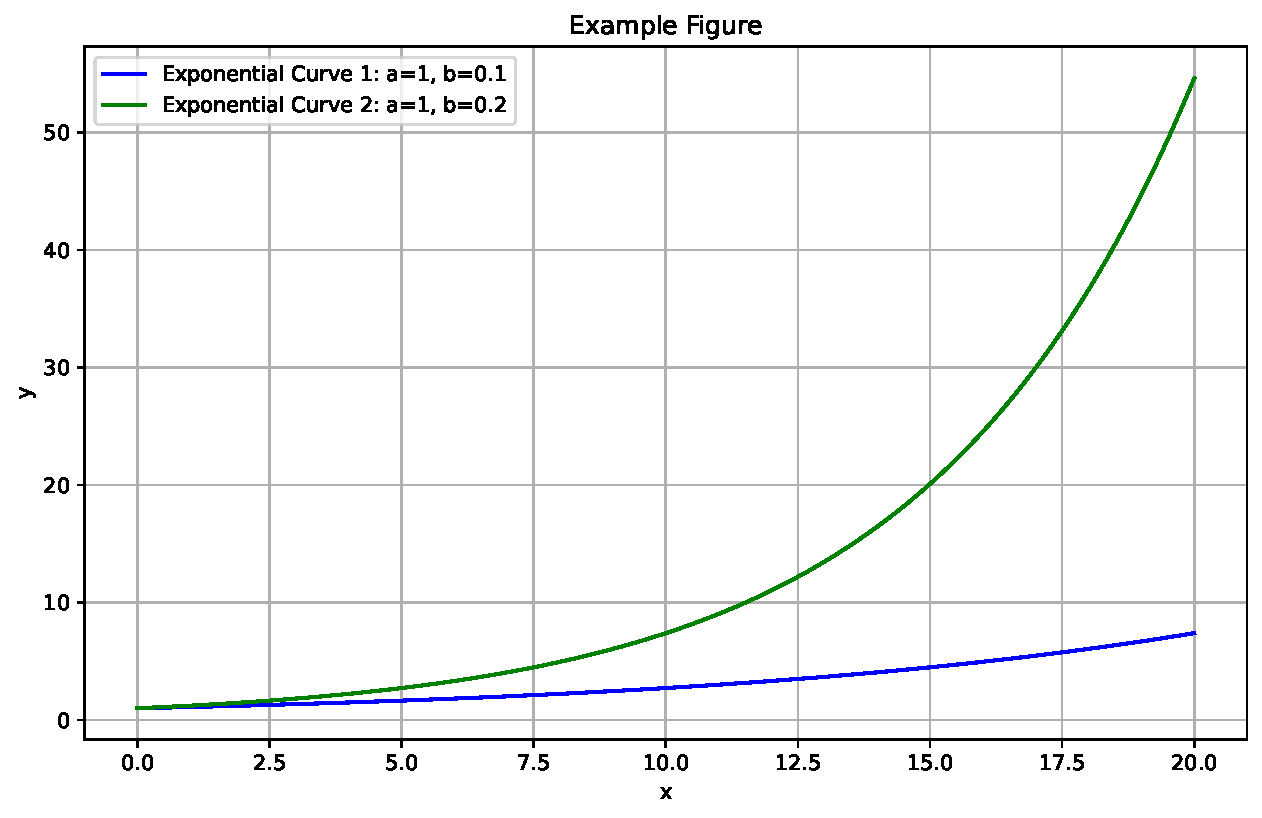
\includegraphics{index_files/figure-pdf/cell-2-output-1.pdf}

}

\end{figure}%

\subsubsection{Figure with R}\label{figure-with-r}

\begin{Shaded}
\begin{Highlighting}[]
\NormalTok{\#| label: fig{-}mtcars}
\NormalTok{\#| fig{-}cap: "MPG vs horsepower, colored by transmission."}
\NormalTok{\#| column: margin}

\NormalTok{library(ggplot2)}
\NormalTok{mtcars2 \textless{}{-} mtcars}
\NormalTok{mtcars2$am \textless{}{-} factor(}
\NormalTok{  mtcars$am, labels = c(\textquotesingle{}automatic\textquotesingle{}, \textquotesingle{}manual\textquotesingle{})}
\NormalTok{)}
\NormalTok{ggplot(mtcars2, aes(hp, mpg, color = am)) +}
\NormalTok{  geom\_point() +}
\NormalTok{  geom\_smooth(formula = y \textasciitilde{} x, method = "loess") +}
\NormalTok{  theme(legend.position = \textquotesingle{}bottom\textquotesingle{})}
\end{Highlighting}
\end{Shaded}

\section{Footnotes}\label{footnotes}

Test footnote 1\footnote{This is the first footnote.} and test footnote
2\footnote{This is the second footnote.}

\section{Asides}\label{asides}

\subsection{Aside with Latex}\label{aside-with-latex}

\marginnote{\begin{footnotesize}

We know from \emph{the first fundamental theorem of calculus} that for
\(x\) in \([a, b]\):

\[\frac{d}{dx}\left( \int_{a}^{x} f(u)\,du\right)=f(x).\]

\end{footnotesize}}

\subsection{Aside with a figure}\label{aside-with-a-figure}



\end{document}
